\chapter{Анализ спектральных данных}
\label{cha:ch_5}

В качестве исследования были обработаны сырые спектральные данные, полученные при одних и тех же
технических условиях системы, в отсутствие пылевого облака, а также в присутствии пылевого облака (см~рис.~\ref{fig:fig34}).

\begin{figure}
    \centering
    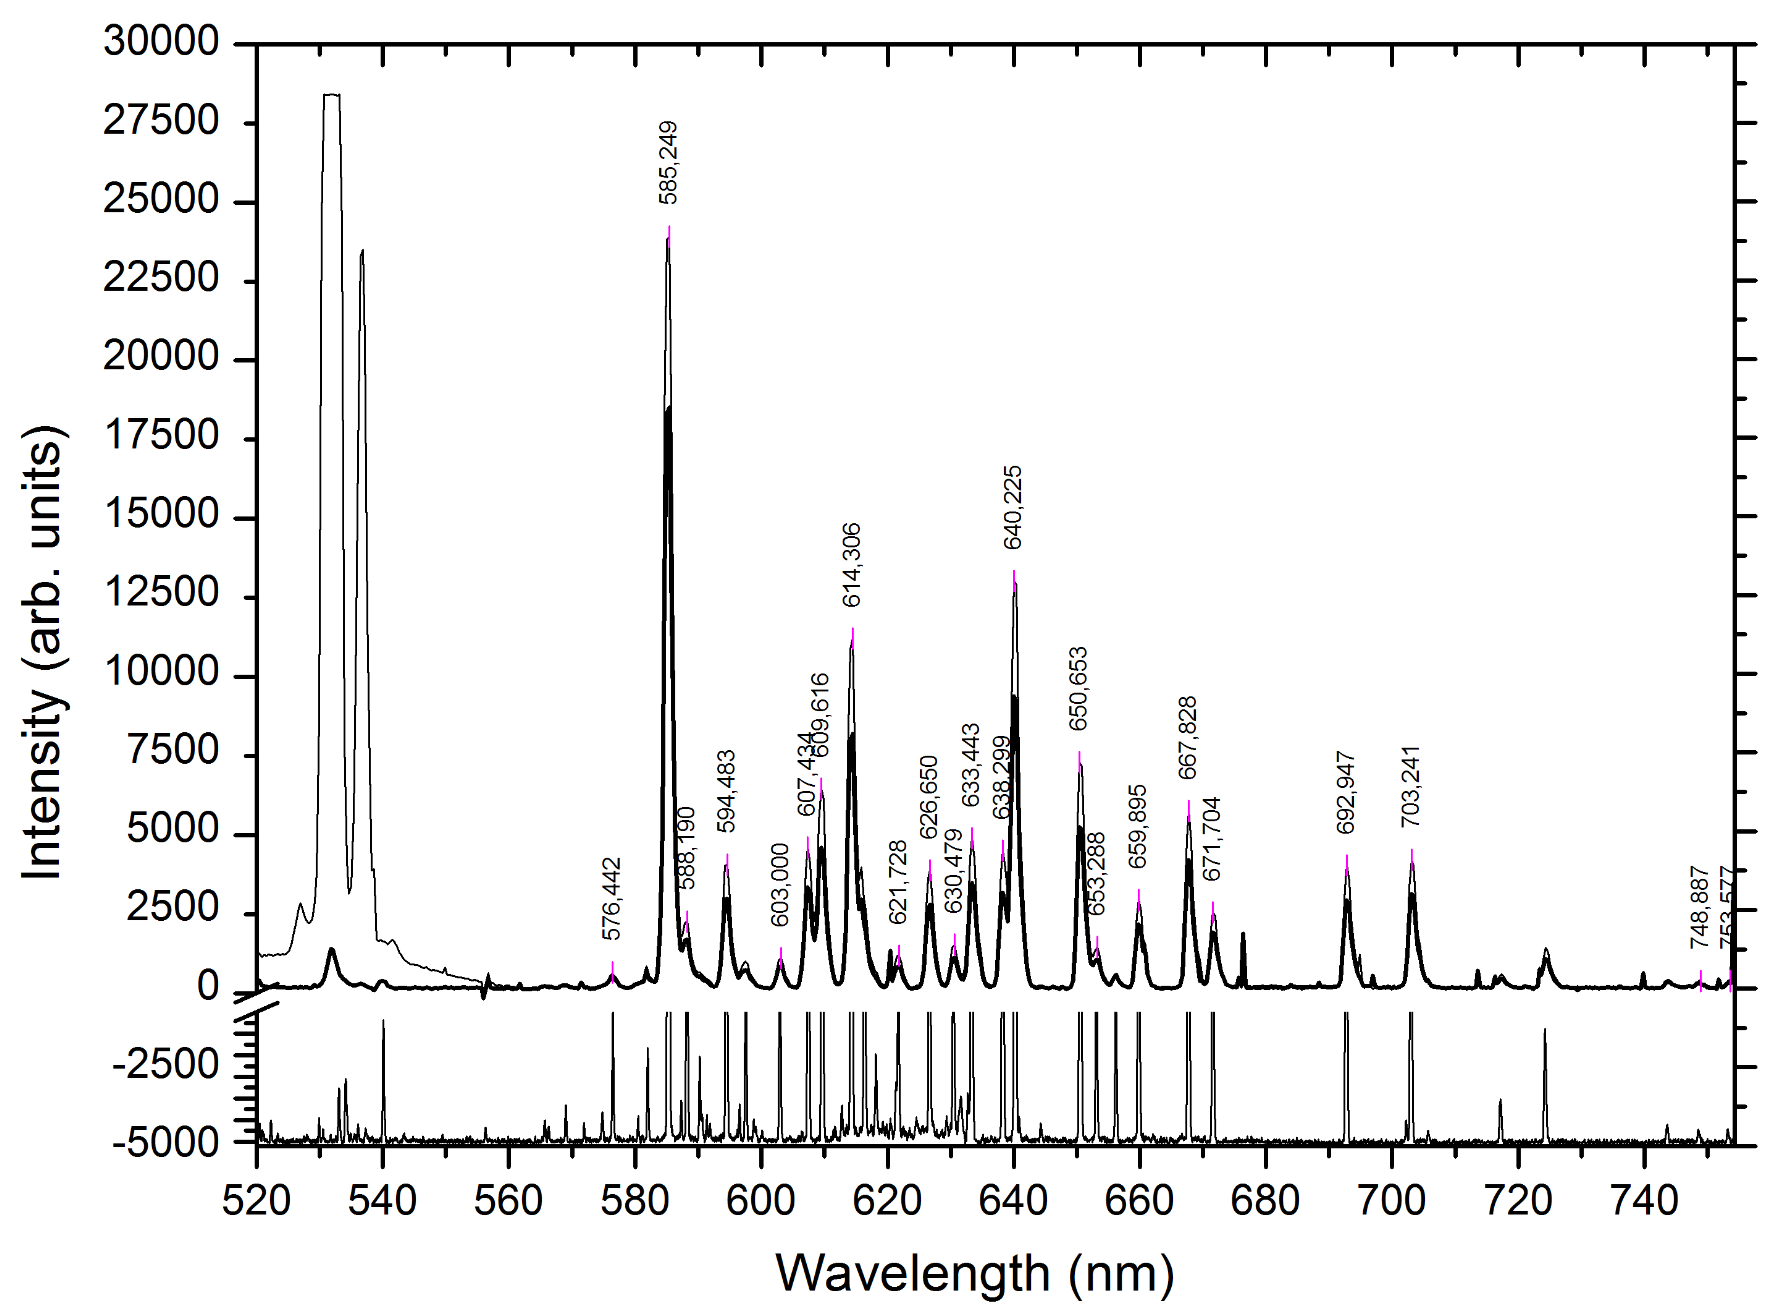
\includegraphics[width=15cm]{figures/fig34}
    \caption{
        Зависимость интенсивности (усл.~ед.) от длины волны (нм). На графике наложены три спектра:
        1. Ниже нуля калибровочный спектр с достоверными линиями неона;
        2. Жирной линией выделен спектр без пылевого облака.
        3. Тонкой линией выделен спектр с пылевым облаком
    }
    \label{fig:fig34}
\end{figure}


Экспериментально было обнаружено увеличение интенсивности спектральных линий при попадании пылевого облака
в газовый разряд неона, причем линии с разными верхними энергетическими уровнями имеют разные значения
отношений интенсивностей (см~рис.~\ref{fig:fig35}).
\begin{figure}
    \centering
    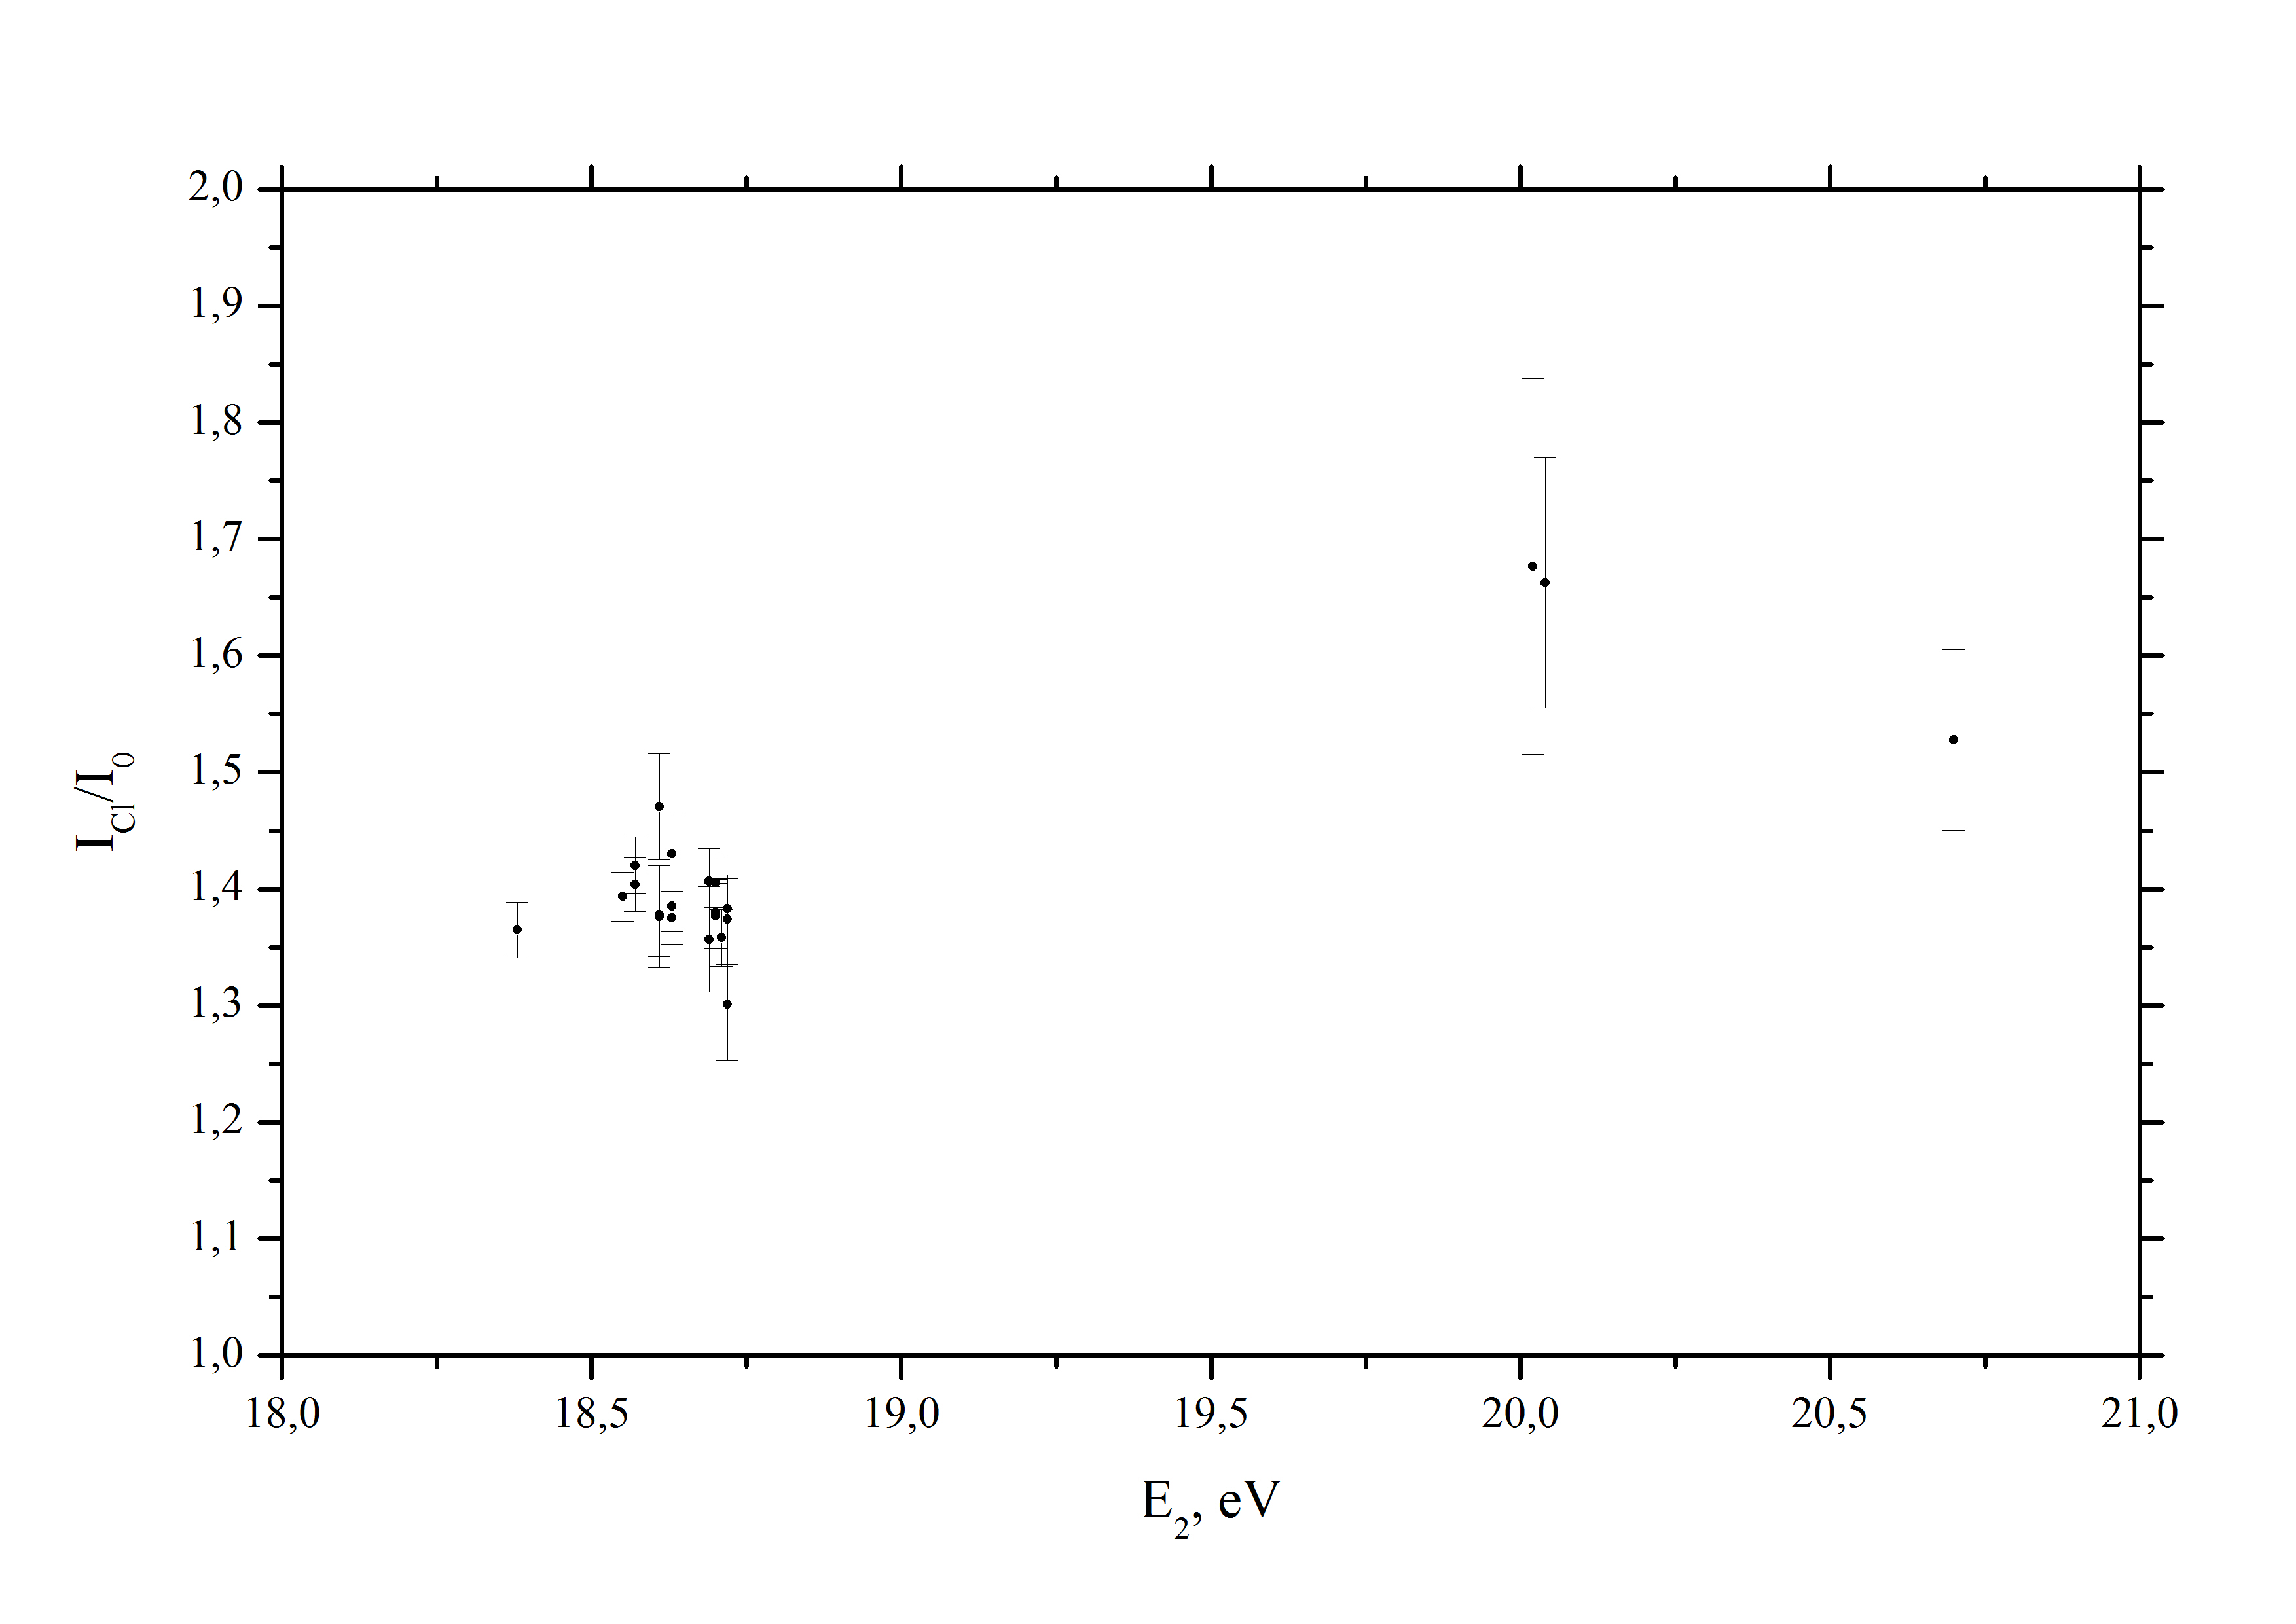
\includegraphics[width=15cm]{figures/fig35}
    \caption{Зависимость отношения интенсивностей спектральных линий неона в присутствии пылевого облака к отсутствию пылевого облака.}
    \label{fig:fig35}
\end{figure}


% [МОЖЕТ СТОИТ ВЫНЕСТИ ДАЛЬНЕЙШИЕ РАССУЖДЕНИЯ В РАЗДЕЛ "АНАЛИЗ СПЕКТРАЛЬНЫХ ДАННЫХ" ???]

Поскольку электроны, имеющие энергию выше пороговой участвуют в неупругих столкновениях с атомами, то ФРЭ должно иметь
двухтемпературное распределение [ССЫЛКА???]. Несложно заметить, что полученные расчетные ФРЭ также имеют двухтемпературный вид:
на рис. {\ref{sub:fig15a}} распределения более менее можно аппроксимировать прямыми линиями со своими электронными
температурами, но хвостовые части (см.~рис~\ref{sub:fig15b}) идеально описываются прямыми линиями. Запишем распределение хвостовой части ФРЭ:
\begin{equation}
    f_{tail}(\epsilon) = e^{-{\epsilon \over T_e}} \Rightarrow ln(f_{tail}) = - {\epsilon \over T_e}
    \label{eq:tail}
\end{equation}

В рамках одного и того же переходного процесса справедливы следующие рассуждения: интенсивность
спектральной линии пропорциональна заселенности верхнего уровня данного перехода, которая в свою очередь
пропорциональна скорости заселения верхнего уровня, т.е.:
\begin{equation}
I(T_e) \sim N^*(T_e) \sim X_{exc}(T_e)  % \sim  \int_{E_{th}}^{\infty} \sigma(\epsilon)f_{tail}(\epsilon)\sqrt{\epsilon}d\epsilon
\label{eq:sim_Te}
\end{equation}

Скорость заселения верхних уровней определяется следующим выражением [МОЖЕТ СТОИТ ВЫНЕСТИ ЕГО В РАЗДЕЛ 1.1 ???]:
\begin{equation}
    X_{exc} (T_e) = \sqrt{2 \over m} \int_{E_{th}}^{\infty} \sigma(\epsilon)f(\epsilon)\sqrt{\epsilon}d\epsilon
    \label{eq:velocity}
\end{equation}
где \math{\sigma (\epsilon)}$~--~сечение неупругих столкновений для переходного уровня в зависимости от энергии;
\math{f (\epsilon)}$~--~ФРЭ.

Используя выражения (\ref{eq:sim_Te}) и (\ref{eq:velocity}) для двух различных конфигураций газового разряда и выбранной
спектральной линии в рамках одного переходного процесса, имеем:
\begin{equation}
{{I_2} \over {I_1}}= {{\int_{E_{th}}^{\infty} \sigma(\epsilon)f_{2}(\epsilon)\sqrt{\epsilon}d\epsilon} \over
{\int_{E_{th}}^{\infty} \sigma(\epsilon)f_{1}(\epsilon)\sqrt{\epsilon}d\epsilon}}
\label{eq:intensities_ratio}
\end{equation}
здесь индексы 1 и 2 обозначают различные конфигурации самосогласованного газового разряда, т.е. при различных осевых
электрических полях. Сечение \math{\sigma}$ и пороговая энергия \math{E_{th}}$ не различаются для двух конфигураций.
Следует отметить, что энергия верхнего уровня влияет на значение отношения интенсивностей, что мы и наблюдаем в эксперименте (см.~рис~\ref{fig:fig16}).

Таким образом, выполнив перебор всех расчетных ФРЭ для различных осевых электрических, можно понять по отношению
интенсивностей спектральных линий и (\ref{eq:intensities_ratio}), какая из ФРЭ описывает новую конфигурацию
газового разряда. Затем по хвостовой части ФРЭ из (\ref{eq:tail}) несложно вычислить и электронную температуру:
\begin{equation}
    T_{e,2} = {ln(f_{tail,1}) \over ln(f_{tail,2})} T_{e,1}
\end{equation}

% ПЕРЕНЕСТИ
\begin{figure}[t]
  \centering
  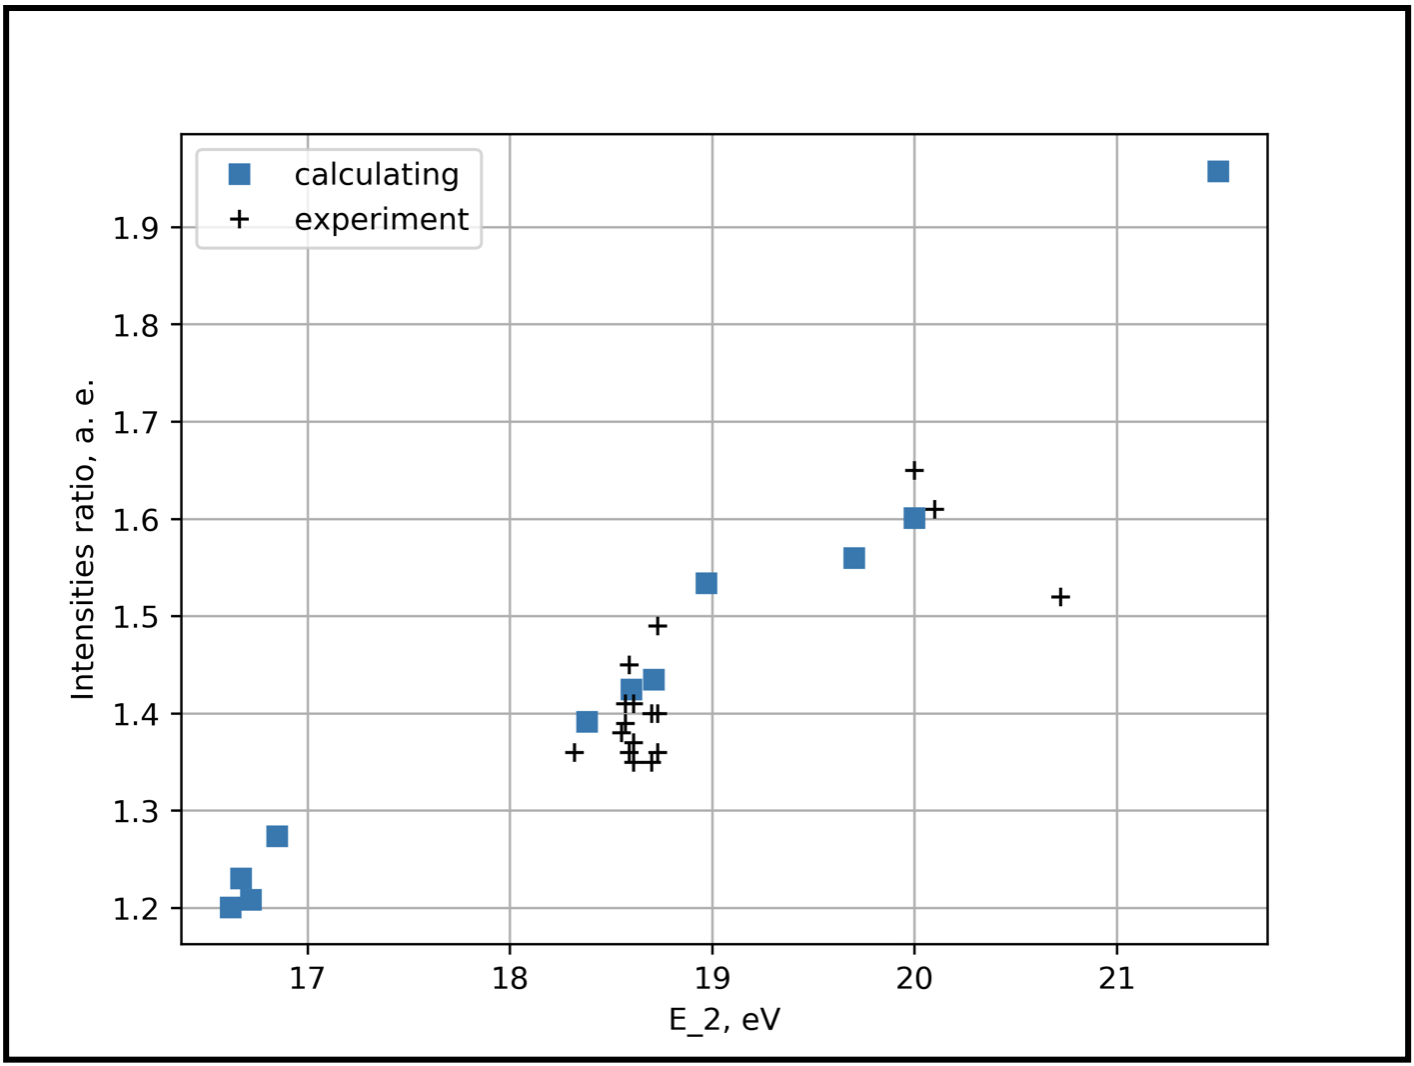
\includegraphics[width=12cm]{figures/fig16}
  \caption{Зависимость ...... .}
  \label{fig:fig16}
\end{figure}
